\documentclass[11pt]{article}
\usepackage{amssymb}
\usepackage{amsmath}
\usepackage{semantic}
\usepackage{listings}
\usepackage{hyperref}
\usepackage{graphicx}
\usepackage{algpseudocode}


\title{Evolution of ORM Systems: Formal Foundations}
\author{Ondrej Macek}

\begin{document}

\maketitle
\begin{abstract}
The evolution of a software is a common issue during software lifecycle. The evolution od code and database are usually separated tasks. We discuss the evolution of software in context of  software created using an object oriented programming language and a relational database. The formal definition of the evolutionary framework is introduced in this paper. Special attention is given to the data stored in databases (instances) and theirs consistency during evolution process.
\end{abstract}

\textbf{Keywords:} data evolution, data migration
\section{Introduction}
The evolution of a software is a common issue during software development. The evolution can occur from many reasons in different stages of software lifecycle. The evolution of a software created using an object oriented programming language and a relational database is usually processed in two steps - as a code refactoring and as a database migration, which is processed as an SQL script. The code refactoring is supported by many IDEs, whereas the database migration is usually processed manually. There are frameworks and tools capable of database evolution, nevertheless these tools are usually not capable to solve complicated migration cases or preserve stored data. Another disadvantage of such an approach to data evolution is the evolution has to be define twice - as a code refactoring and as a database migration.

There are three main goals of our evolutionary framework: 1) provide one source of evolution definition for both: code and database 2) provide a tool, which will be able to preserve stored data 3) minimize the manual work during data evolution in a software.

This paper provides a formal definition of such a framework, which is based on model driven architecture. There are defined models representing an application and database in this paper, together with transformations which are able to perform an evolution of the whole software and preserve data.

The paper is organized as follows: in Section \ref{sec:evoIntro} the concept of ORM software and its evolution is discussed, then models of application and database are introduced in Section \ref{sec:appModel} and in Section \ref{sec:dbModel}, the ORM is defined in Section \ref{sec:orm} and the evolutionary transformations are defined in Section \ref{sec:eorm}.

\section{ORM Software}
\label{sec:evoIntro}
\begin{figure}
\centering
	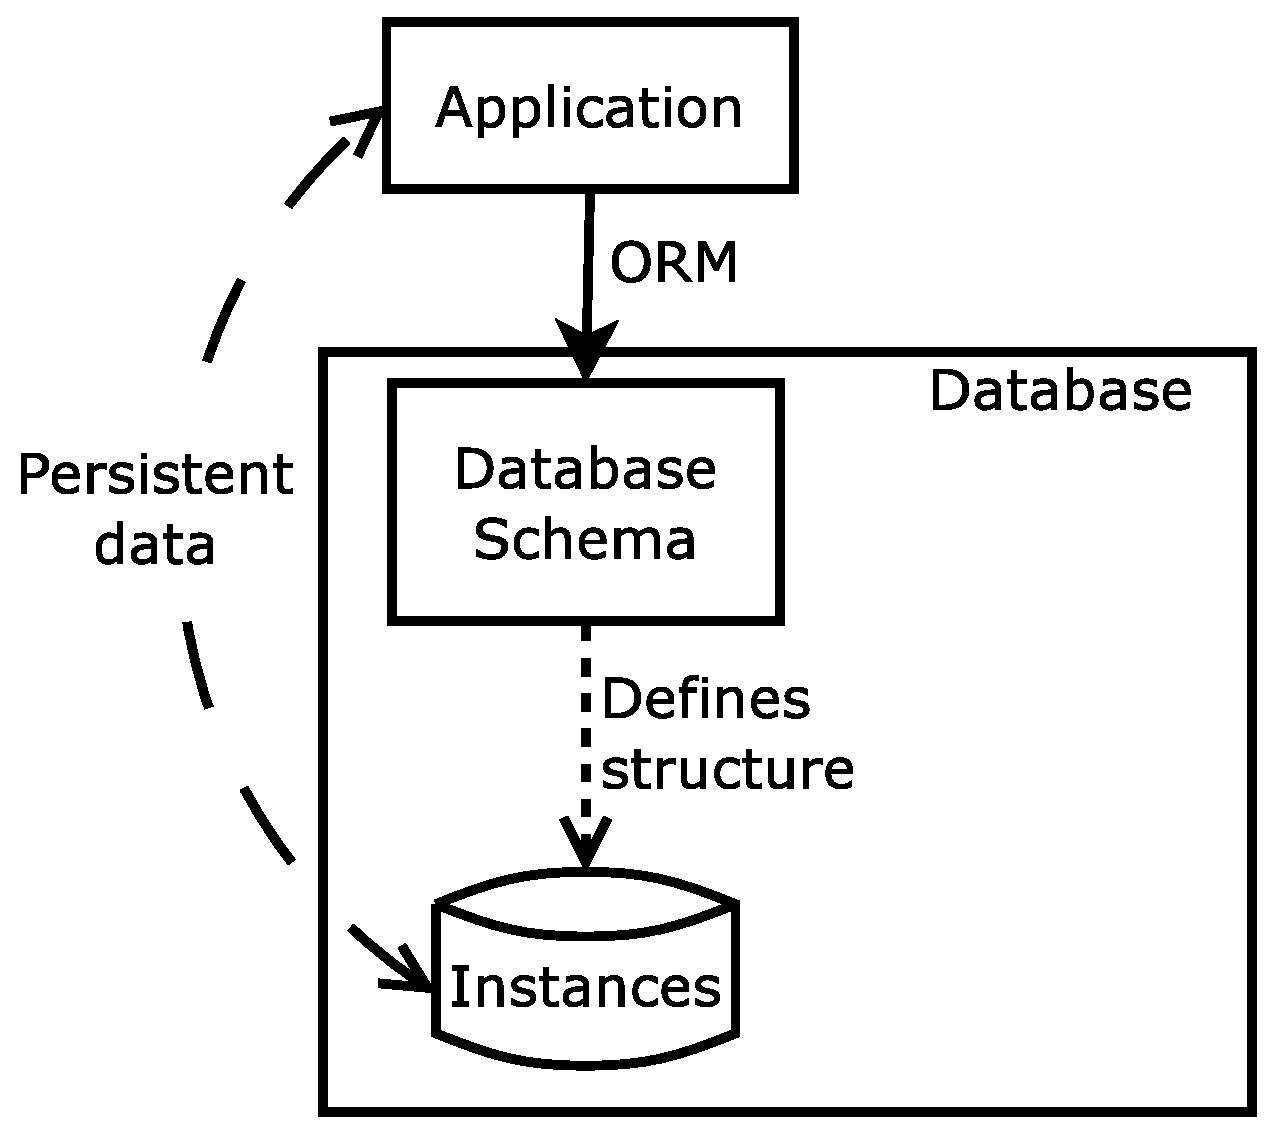
\includegraphics[scale=0.3]{./images/system}
	\caption{The model of one generation of an ORM system consists of application persistent layer and relational database for storing instances.}
\label{fig:appStructure}
\end{figure}
A software implemented using an object-oriented language, which uses relational database as a data storage (as illustrated in the Figure \ref{fig:appStructure}) is object of interest of this paper. There are three important components of such a software: application (its persistent layer concretely), database (consisting of database schema and stored data) and an ORM (we will use $\rho$ as a symbol for ORM), therefore we define a software as a triple:
\begin{align*}
	\mathbf{software} = < Application, Database, \rho > \\
	sw : Applications \times Databases \times ORM \rightarrow Software \\ \\
	\mathbf{application} : Software \rightarrow Application \\
	application(sw(a, d, \rho)) = a \\ \\
	\mathbf{database} : Software \rightarrow Database \\
	database(sw(a, d, \rho)) = d \\
	a \lhd Application, d \lhd Database
\end{align*}
The software definition above introduce the first type used in this paper. The notation $a \lhd Application$ indicates the variable $a$ has the type $Application$.

The software has to be in consistent state so its users could have benefit from its usage. The state of the software is defined to communicate the sate of the software to its user. The components of a software (application and database) are transformed likewise, thus the state is defined for them too.
\begin{align*}
 	\mathbf{state} = Consistent\; s \: | \: Inconsistent \; s,  \\	s \lhd Software \vee s \lh Application \vee s \lhd Database
\end{align*}
Before the definition of the software consistency is provided, the notation of function transcription has to be introduced. Usually the definition of a function consists of two parts - an effect of the function and conditions when the effect occurs We decide to use following transcription, to simplify the notation and to improve understanding of functions:
\begin{align*}
f(x) =   \inference{conditions}{effect}
\end{align*}
The function querying the state (it means consistency) of a software is defined as:
\begin{align*}
 	\mathbf{consistent} : State \rightarrow Boolean \\
 	consistent(s) = \begin{cases}
 		\inference{s = Consistent(s)}{true}\\\\
 		\inference{s = Inconsistent(s)}{false}\\
 \end{cases}\\
 s \lhd State
\end{align*}
The consistency of application and database is discussed later in this paper. The definition of software state only is provided:
\begin{align*}
	\mathbf{state} : Software \rightarrow State \\
	state(s) = \begin{cases}
 		\inference{consistent(application(s)) \wedge \\ consistent(database(s)) \\ \wedge \rho(application(s)) = database(s)}{Consistent \; s}\\ \\
 		\inference{otherwise}{Inconsistent \; s}
 	\end{cases} \\ 
 	s \lhd Software
\end{align*}

\subsection{Software Evolution}
\begin{figure}
\centering
	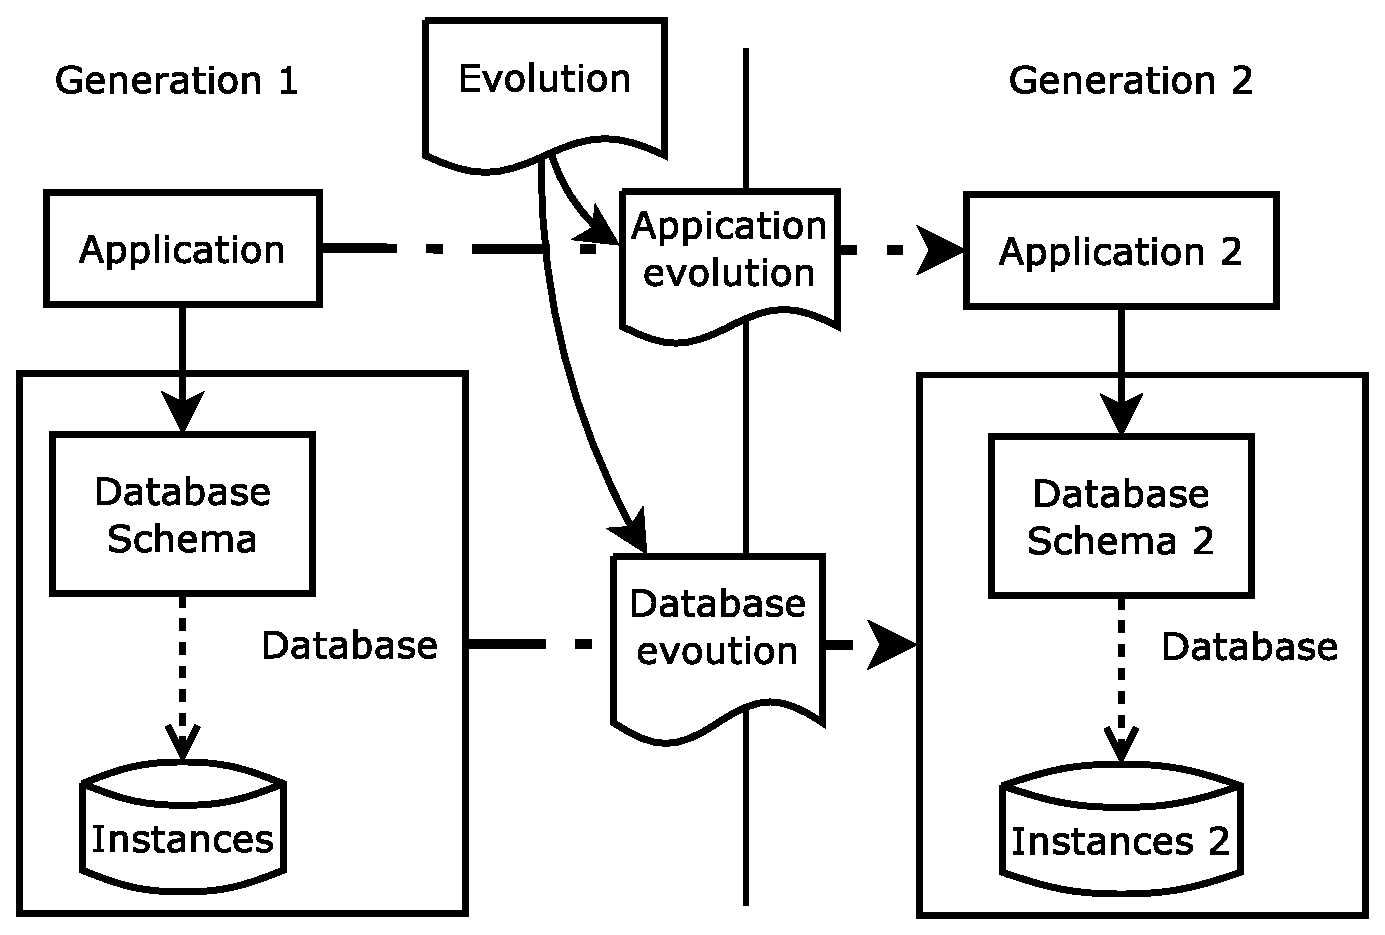
\includegraphics[scale=0.4]{./images/evolution_simple}
	\caption{The evolution of data changes the system on all levels. The figure shows all the components of the evolution process.}
	\label{fig:evolution}
\end{figure}
The evolution of a software is a transformation from one consistent state to another one. These states are called generations of the software and the function which changed the state of a software are called transformations. The evolution consists of change in application and in database as shown in the Figure \ref{fig:evolution}. We focus on situations when the evolution is initiated on the application level (as code refactoring), thus the transformation are designed to conform to the refactoring cases. However a case when the evolution begins on database level is also possible (eg. as a result of database optimization) it is not considered in this paper. 

The evolution of the whole software has to be processed on the both software components - application and database. It means there is a set of application transformations called $AppT$ and a set of database transformations called $DbT$. Because there are needed different parameters for application and database evolution the evolution of database can not be derived from application evolution only. Thus the set of transformation called $E$ is defined to evolve the whole software together with mappings $\Psi$ between $E$ and $AppT$ and $\Phi$ between $E$ and $DbT$ is defined:
\begin{align*}
\Psi : E \rightarrow AppT \\
\Phi : E \rightarrow DbT
\end{align*}
The set $E$ containing the evolution transformations of a software mets our first goal - a single source of data evolution for the whole software.

The application of a transformation on a software state (evolution) is marked by the $\oplus$ operator:
$$\oplus : State \times E \rightarrow State $$
and similarly the $\circ$ and the $\bullet$ operators for evolving application and database:
\begin{align*}
\circ : State \times AppT \rightarrow State \\
 \bullet : State \times DbT \rightarrow State
\end{align*}
The definition of the evolving operator is inspired by the monads (as used e.g. in Haskell programming language) so the state of the software can be passed from one evolution step to another, which helps us to concatenate evolution transformations.
\begin{align*}
 state(s) \oplus t = \begin{cases}
 	\inference{! consistent(state(s))}{u} \\ \\
 	\inference{consistent(state(s))}{state(sw(\Psi(s, t), \Phi(s,t))} 
\end{cases}\\ 
s \lhd Software, t \in E
\end{align*}
\begin{align*}
 state(a) \circ e = \begin{cases}
 	\inference{!\;consistent(state(a))}{a} \\ \\
 	\inference{consistent(state(a))}{e(a)} 
\end{cases}\\ 
a \lhd Application, e \in AppT
\end{align*}
\begin{align*}
 state(d) \bullet e = \begin{cases}
 	\inference{!\;consistent(state(d))}{d} \\ \\
 	\inference{consistent(state(d))}{e(d)} 
\end{cases}\\ 
d \lhd Application, e \in DbT
\end{align*}

\section{Software Model}
The model of an ORM software consists of three parts - an application model, a database model and an ORM. The model of application and database creates a type system for both ORM and evolutionary transformations.

The definitions of all parts assume a set $Label$ exists which contains all possible identifiers and each modeled entity is unambiguously identified in the model. Next there is a set $Values$ containing all possible values, which can be used in the model. 

\subsection{Application Model}
\label{sec:appModel}
The application model represents an application persistent layer created using object oriented language and functions which can alter the model. 
\subsubsection{Application Structure}
Each instance in an application is defined according to some class - the class defines the structure of its instances and relationships between them an the rest of the application. The instances are stored in the relational database in our case, therefore we define only the structure of classes in our model. 
\begin{align*}
  \mathbf{Application} = < Class* > \\ 
  \mathbf{app} : Class* \rightarrow  Application \\ \\
  \mathbf{classes} : Application \rightarrow Class* \\
  classes(app(cs)) = cs  \\\\
  \mathbf{class} : Label \times Application \rightarrow Class   \\ 
  class(l, a) = c, c \in classes(a) \wedge name(c) = l \\ \\
  l \in Label,a \lhd Applications, cs = Class* 
\end{align*}

\paragraph{Class} Class represents a basic structural unit in the application model. It has a unique name, one or more properties and it can be associated to other classes in the application. 
\begin{align*}
	\mathbf{Class} = <label, Property*, Association*> \\
	\mathbf{cl} : Label \times Property* \times Association* \rightarrow Class \\\\
	\mathbf{name} : Class \rightarrow Label \\
	name(cl(l, props, assocs)) = l \\ \\
	\mathbf{properties} : Class \rightarrow Property* \\
	properties(cl(l, props, assocs)) = props \\ \\
	\mathbf{associations} : Class \rightarrow Association* \\	associations(cl(l, props, assocs)) = assocs \\ 
	l \in Label, props \lhd Property*, assocs \lhd Association*
\end{align*}
Three more function are defined to obtain information about a class - function $primitives$ returns all properties of the class which represent a single value, whereas function $collections$ returns all properties representing collection of values. The last function called $associated$ determine if a class is associated by any other class in an application.
\begin{align*}
	\mathbf{primitives} : Class \rightarrow Property* \\	primitives(cl(l, props, assocs)) = props', \\ props' \subset props,  \forall p \in props' : cardinality(p) \leq 1 \\ \\
	\mathbf{collections} : Class \rightarrow Property* \\	collections(cl(l, props, assocs)) = props', \\ props' \subset props, \forall p \in props' : cardinality(p) > 1 \\ \\
	\mathbf{associated} :  Label \times Application \rightarrow Boolean \\
  	associated(l,a) = \begin{cases}
  		\inference{\exists c \in classes(a) \wedge \exists e \in associations(c) : \\ reference(e) = l
  	}{ true } \\\\
 		false
 	\end{cases} \\ \\
	l \in Label, props = Property*, assocs = Association*,a \lhd Applications
\end{align*}
	 
\paragraph{Property} Property represents a feature of a class which is represented as a primitive type. The property can be mandatory, can have a default value and according to its cardinality it can represent a single value or a collection of values. The $owningClass$ function returns the class in the model which owns the property.
\begin{align*}
	\mathbf{Property} = <label, AppType, DefaultValue, Cardinality, Mandatory> \\
	\mathbf{prop} : Label \times AppType \times String \times \mathbb{N^{*}} \times Boolean \rightarrow Property \\ \\
	\mathbf{name} : Property \rightarrow Label \\
	name(prop(l, t, val, n, m)) = l \\ \\
	\mathbf{type} : Property \times AppType \\
	type(prop(l, t, val, n, m)) = t \\ \\
	\mathbf{cardinality} : Property \rightarrow \mathbb{N^{*}} \\
	cardinality(prop(l, t, val, n, m)) = n \\ \\
	\mathbf{mandatory} : Property \rightarrow Boolean \\
	mandatory(prop(l, t, val, n, m)) = m  \\ \\
	\mathbf{owningClass} : Property \times Application \rightarrow Class  \\ 	
	owningClass(p, a) = \inference{\exists c \in classes(a) \wedge p \in properties(c)}{c}  \\ \\
	l \in Label, t \lhd AppType, val \in Values, n \in \mathbb{N^{*}}, m \in Boolean 
\end{align*}

\paragraph {Association} Associtation represents a connection between two classes. It has a unique name and the reference is represented by the label of referenced class. The class which owns the association is consider to be the starting class of an association, referenced class is consider to be the ending class of an association. The cardinalities defines the multiplicity of both association ends.
\begin{align*}
	\mathbf{Association} = <label, classRef, startCardinality, endCardinality> \\
	\mathbf{assoc} : Label \times Label \times \mathbb{N} \times \mathbb{N} \rightarrow Association\\ \\
	\mathbf{name} : Association \rightarrow Label \\
	name(assoc(l, ref, n_1, n_2)) = l\\ \\
	\mathbf{reference} : Association \rightarrow Label \\
	reference(assoc(l, ref, n_1, n_2)) = ref\\ \\
	\mathbf{startCardinality} : Association \rightarrow \mathbb{N} \\
	startCardinality(assoc(l, ref, n_1, n_2)) = n_1\\ \\
	\mathbf{endCardinality} : Association \rightarrow \mathbb{N} \\
	endCardinality(assoc(l, ref, n_1, n_2)) = n_2 \\ \\
	\mathbf{owningClass} : Association \times Application \rightarrow Class  \\
	owningClass(as, a) = \inference{\exists c \in classes(a) \wedge as \in associations(c)}{c}  \\ \\	
	l, ref \in Label,  n_1, n_2 \in \mathbb{N}, as \lhd Association
\end{align*}


%TODO: variable types

\paragraph{Application type} Application type ($AppType$) represents primitive type in the application. There are usually defined types such as String, Integer, Boolean etc. in contrast there is only one type in our model, because we focus on structural and data changes and type casting operations are not important for us. The only $AppType$ type is called $APPSTRING$.
\begin{align*}
\mathbf{AppType} = APPSTRING
\end{align*}

\subsubsection{Application consistency}
The application consistency is based on the structural consistency of its model. Violation of structural consistency are name collisions and non-existing references in associations. The state of an application is:
\begin{align*}
	state(a) = \begin{cases}
	\inference{\forall c_1, c_2 \in classes(a) : name(c_1) \neq name(c_2) \\ \wedge \forall p_1, p_2 \in properties(c_1) : name(p_1) \neq name(p_2) \\ \wedge \forall a_1, a_2 \in associations(c_1) : name(a_1) \neq name (a_2) \\ \wedge \forall a \in associations(c_1) : \exists c \in classes(a) \wedge name(c) = reference(a) }{Consistent \; a}\\\\
 	Inconsistent \; a
 	\end{cases}\\
	a \lhd Application
\end{align*}


\subsection{Database Model}
\label{sec:dbModel}
The relational database consists of database schema which defines the structure of the database and data, which in our ORM system represents stored instances. The database is defined as a tuple:
\begin{align*}
	\mathbf{Database} = < Table*, Row*> \\
	\mathbf{db} : Tables \times Rows \rightarrow Database \\ \\
	\mathbf{tables} : Database \rightarrow Tables \\
	tables(db(tabs, rs)) = tabs \\ \\
	\mathbf{rows} : Database \rightarrow Rows \\
	rows(db(tabs, rs)) = rs \\ \\
	tabs = Table*, rs = Row*, l \in Label,d \lhd Database
\end{align*}
\paragraph{Table} Table represents a basic concept of database schema. It has a unique name, one or more columns and it can be related to other tables in the schema by foreign keys. Rows in the table represents stored data.
\begin{align*}
	\mathbf{Table} = <label, primaryKey, Column*, ForeignKey*>\\
	\mathbf{tab} 	: Label \times PrimaryKeys \times Columns \times ForeignKeys \rightarrow Table \\ \\
	\mathbf{name} : Table \rightarrow Label  \\
	name(tab(l, pk, cols, fks)) = l \\ \\
	\mathbf{primaryKey} : Table \rightarrow PrimaryKeys  \\
	primaryKey(tab(l, pk, cols, fks)) = pk \\ \\
	\mathbf{columns} : Table \rightarrow Columns  \\
	columns(tab(l, pk, cols, fks)) = cols \\ \\
	\mathbf{foreignKeys} : Table \rightarrow ForeignKeys  \\
	foreignKeys(tab(l, pk, cols, fks)) = fks \\ \\
l \in Label, pk \lhd PrimaryKey, cols = Column*, fks = ForeignKey*
\end{align*}

\paragraph{Column} Column defines data values and types which can be part of a table record.
\begin{align*}
	\mathbf{Column} = <label, DbType, DefaultValue, Constraint*> \\
	\mathbf{col} : Label \times DbType \times String \times Constraints \rightarrow Column \\ \\
	\mathbf{name} : Column \rightarrow Label  \\
	name(col(l, t, val, cons)) = l  \\ \\
	\mathbf{type} : Column \rightarrow DbType  \\
	type(col(l, t, val, cons)) = t  \\ \\
	\mathbf{constraints} : Column \rightarrow Constraints  \\
	constraints(col(l, t, val, cons)) = cons  \\ \\
	\mathbf{owningTable} : Column \times Database \rightarrow Table  \\
	owningTable(c, d) = \inference{\exists tab \in tables(d) \wedge c \in columns(tab)}{tab} \\ \\
l \in Label, t \lhd DbType, val \in Values,\\ cons \lhd Constraint*, c \lhd Column,d \lhd Database
\end{align*}

\paragraph{Foreign key} Foreign key is a reference to another table's primary key, it has an unique name and it can be constrained. The value of a foreign key is $\varnothing$ or a non-zero natural number.
\begin{align*}
	\mathbf{ForeignKey} = <label, tableRef, Constraint*> \\ 
	\mathbf{fk} : Label \times Label \times Constraints \rightarrow ForeignKey \\ \\
	\mathbf{name} : ForeignKey \rightarrow Label \\
	name(fk(l, tRef, cons)) = lab  \\ \\
	\mathbf{reference} : ForeignKey \rightarrow Label  \\
	reference(fk(l, tRef, cons)) = tRef  \\ \\
	\mathbf{constaints} : ForeignKey \rightarrow Constraint*  \\
	constaints(fk(l, tRef, cons)) = cons  \\ \\
	\mathbf{owningTable} : ForeignKey \times Database \rightarrow Table  \\
	owningTable(fk, d) = \inference{\exists tab \in tables(d) \wedge fk \in foreignKeys(tab)}{tab}\\\\
	l, tRef \in Label, cons \lhd Constraint*,d \lhd Database, fk \lhd ForeignKey
\end{align*}


\paragraph{Primary key} Primary key is unambiguous identifier of a record in a table. The primary key is always provided (automatically generated) by the database as a non-zero natural number. Primary key is always defined with constraints $NOTNULL$ and $UNIQUE$. 
\begin{align*}
	\mathbf{PrimaryKey} =  < label > 	\\
	\mathbf{pk} : Label \rightarrow PrimaryKey
\end{align*}

\paragraph{Data Types} Database data types $DbType$ represents primitive types in the database. There are usually defined types such as Varchar, Integer, Boolean etc. There is only one type of column values defined in the model called $DBSTRING$. Next the $DBN$ type is defined for the values of keys.
\begin{align*}
	\mathbf{DbType} = DBSTRING | DBN
\end{align*}

\paragraph{Constraints} There are two types of constraints defined in the model. Both constraints are column constraints - first constraint defines non-empty columns, second constraint defines there has to be unique records in a column or foreign key.
\begin{align*}
	\mathbf{Constraint} = NOTNULL \; | \; UNIQUE 
\end{align*}

%%%%%%%%%%%%%%%%%%%%%%%%%%%%%%

\paragraph{Stored Data} A database consists not only from schema but also from data which are represented as rows in a table. A table row in our model is a tuple consisting of value pairs, which represents concrete value of concrete column. Each row contains a name of a table it belongs to.
\begin{align*}
	\mathbf{Row} = < refTable, pkValue, pair* > \\
	\mathbf{row} : Label \times Pairs \rightarrow Row \\ \\
	\mathbf{refTable} : Row \rightarrow Label \\
	refTable(row(l, n, ps) = l \\ \\
	\mathbf{pairs} : Row \rightarrow Pair* \\
	pairs(row(l, n, ps)) = ps \\ \\
	\mathbf{pkValue} : Row \rightarrow N \\
	pkValue(row(l, n, ps)) = n \\ \\
	 l \in Label, ps = Pair*, n \in N
\end{align*}
The value stored in concrete column of the row is represented by a pair, where the $refCol$ is a name of the column, a foreign key or its primary key and $value$ represents concrete value .
\begin{align*}
	\mathbf{Pair} = < refCol, value > \\
	[Label \times Value] \rightarrow Pair\\ \\
	\mathbf{reference} : Pair \rightarrow Label \\
	reference([l,val]) = l \\ \\
	\mathbf{value} : Pair \rightarrow Value \\ 
	value([l,val]) = val \\ \\
	l \in Label, val \in Value
\end{align*}
The definition of data allows definition of function $contains$ which verify if the table contains data in context of concrete database and $instantiated$, which search for instances of a class with given name and returns true if there are rows for the table in the database.
\begin{align*}
	\mathbf{contains} : Table \times Database \rightarrow Boolean \\
	contains(t, d) = \begin{cases}
			\inference{\exists r \in data(d) : refTable(r) = name(t) }{true} \\ \\
		 	false
 		\end{cases} \\ \\
 l \in Label, ps = Pair*, t \in tables(d), d \lhd Database
\end{align*}
\begin{align*}
	\mathbf{tableData} : Label \times Row* \rightarrow Row* \\
	tableData(l, r) = \begin{cases}
 		\inference{r = \varnothing}{\varnothing} \\
 		\inference{|r| > 1}{tableData(head(r)) \cup tableData(tail(r))}\\ \\
 		\inference{|r| = 1 \wedge refTable(r) = l}{r}\\\\
 		\inference{|r| = 1 \wedge refTable(r) \neq l}{\varnothing}
 \end{cases} \\ \\
	r \lhd Row*, l \in Label
\end{align*}
\begin{align*}
	\mathbf{instantiated} : Class \times Software \rightarrow Boolean \\
	instantiated(c, s) = \begin{cases} \inference{\exists t \in tables(database(s)) : name(t) = name(c) \\ \wedge contains(t, database(s))}{true} \\ \\
  false
 \end{cases} \\ \\
	 c \in classes(application(s)), s \lhd Software 
\end{align*}

\subsubsection{Database consistency}
The database consistency is founded on the consistency of structure and consistency between structure and stored values. The conditions for structure consistency are similar as for application structure. The consistency between structure and data is:  each row in a database  refers to a table in database schema and it has to have the structure corresponding to the one defined by a table, moreover the column and foreign key constrains has to be fulfilled  otherwise the database is inconsistent. The consistency of database is:
\begin{align*}
	\mathbf{consistent} : Database \rightarrow Boolean \\
	state(d) = \begin{cases}
 		\inference{ \forall t_1, t_2 \in tables(d) : name(t_1) \neq name(t_2) \\ \wedge \forall c_1, c_2 \in columns(t_1) : name(c_1) \neq name(c_2) \\ \wedge \forall f_1, f_2 \in foreignKeys(t_1) : name(f_1) \neq name (f_2) \\ \wedge \forall f \in foreignKeys(t_1) : \exists t \in tables(d) \wedge name(t) = reference(f) \\ \wedge \forall r \in data(d): ( \exists t \in tables(d) : reference(r) = name(t) \\ \wedge \forall p \in pairs(r) :\\ \exists u \in columns(t) \cup foreignKeys(t) \cup primaryKey(t) : \\ reference(p) = name(u) \\ \wedge \forall e \in columns(t) \cup foreignKeys(t) \\ \wedge NOTNULL \in constrain(e) : \exists q \in pairs(r) \wedge name(e) = reference(q)) \\ \wedge \forall g \in columns(t) \cup foreignKeys(t) \\ \wedge UNIQUE \in constrain(g) : \\ \forall u_1, u_2 \in rows(t) : \\ value(pairByName(name(g), u_1) \neq value(pairByName(name(g), u_2) }{true}
 	\\ \\
 	false
 \end{cases}
\end{align*}
 

\subsection{Object-Relational Mapping}
\label{sec:orm}
There are defined functions for object-relational mapping used in this paper. The mapping function itself are not able to create a database from the application as they are mentioned to be used together with evolutionary transformations introduced in section \ref{sec:transformations}.

\paragraph{Mapping of Application} The goal of ORM is usually to determine how an instance is stored in the database. The ORM maps the structure of application classes to database schema. The assumption is a software is evolved continuously and evolutionary transformations produces consistent software, nevertheless to verify consistency of a software we need mapping between an existing application structure and database schema. 
\begin{align*}
	\mathbf{\rho_{app}} : Application \rightarrow Database\\
	\rho_{app}(a) = \inference{state(a) = Consistent a}{\begin{gathered}
	db(\varnothing) \bullet addTable(classes(a)) \\ 
	\bullet (\forall c \in classes(a), p \in properties(c) : addProperty(name(c), p) \\
	\bullet (\forall c \in classes(a), e \in associations(c) : addAssociaiton(name(c), e) 
\end{gathered}}
\end{align*}


\paragraph{Mapping of Types} The mapping of types assumes a bijection between application types and database types, otherwise there has to be additional information for type mapping. We focus on structural and data change therefore there is only one type of values in both our models. The mapping is then straightforward:
\begin{align*}
	\mathbf{\rho_{t}} : AppType \rightarrow DbType  \\
 	\rho_{t}(APPSTRING) = DBSTRING 
\end{align*}

\paragraph{Mapping of Classes} The class is mapped into a table with  automatically created primary key. The primary key is always created with name Id and of the $\mathbb{N^{*}}$ type. The properties and associations has to be mapped separately.
\begin{align*}
	\mathbf{\rho_{c}} : Class*  \rightarrow Table* \\
	\rho_{c}(c) = \begin{cases}
		\inference{c = \varnothing}{\varnothing}\\\\
		\inference{|c| = 1}{table(name(c), primaryKey("Id"), \varnothing, \varnothing)}  \\ \\
		\inference{|c| > 1}{\rho_c(head(c)) \cup \rho_c(tail(c))}
 \end{cases}\\
 c \lhd Class
\end{align*}

\subsubsection{Mapping of Properties}
There are two kinds of properties - primitive property with cardinality equal to one is mapped to a column; second kind - collection with cardinality greater than one is mapped to table, thus there are two mapping cases. When the property is mandatory the $NOTNULL$ constraint is added to the column with property value. 

There can occur name collision during mapping in case there are more classes with property representing collection. To avoid that the mapping changes the name of the table representing a collection.
\begin{align*}
	\mathbf{\rho_p} : Property* \rightarrow Column* \\ \\
	\rho_{sp}(p) = \begin{cases}
		\inference{p = \varnothing}{\varnothing}\\
		\inference{|p| > 1}{\rho_{sp}(head(p)) \cup \rho_{sp}(tail(p))}\\\\
 		\inference{cardinality(p) = 1 \wedge !\;mandatory(p)
 			\\ \wedge \exists t : t = table(name(owningClass(p)), d) 
		 }{\begin{gathered}
	  		column(name(p), \rho_t(type(p)), \varnothing )
		\end{gathered}} \\ \\
  		\inference{cardinality(p) = 1 \wedge mandatory(p)
			 \\ \wedge \exists t : t = table(name(owningClass(p)), d)
			\\ \wedge \not instanciated(owningClass(p))
		}{\begin{gathered}
 	 		column(name(p), \rho_t(type(p)), NOTNULL ) \\ 
		\end{gathered}}
	\end{cases}\\
	p \lhd Property
\end{align*}
\begin{align*}
	\mathbf{\rho_p} : Property* \rightarrow Table* \\ \\
	\rho_{cp}(p) = \begin{cases}
		\inference{p = \varnothing}{\varnothing}\\
		\inference{|p| > 1}{\rho_{cp}(head(p)) \cup \rho_{cp}(tail(p))}\\\\
     	\inference{cardinality(p) > 1 \wedge !\;mandatory(p) \\ 
     		\wedge 	\exists t : t = table(name(owningClass(p)), d)
     		}{\begin{gathered}
     			table(name(t)+name(p), primaryKey("Id"), \\ column("value", \rho_t(type(p)), \varnothing), \\ foreignKey(name(p), 			name(owningClass(p)), NOTNULL) \\
    	\end{gathered}}\\ \\
     	\inference{ cardinality(p) > 1 \wedge mandatory(p) \\ 
     		\wedge \exists t : t = table(name(owningClass(p)), d) 
     		}{\begin{gathered}  
     			table(name(t)+name(p), primaryKey("Id"), \\ 
     			column("value", \rho_t(type(p)), NOTNULL), \\ 			foreignKey(name(p), name(owningClass(p)), NOTNULL)
    	 \end{gathered}}
 	\end{cases}\\
 	p \lhd Property
\end{align*}

\paragraph{Mapping of Associations} An association is mapped into database as a foreign key in table representing associated class or as a table in case the association cardinality is one to many or many to many. Thus there are two mapping cases as for properties and the same solution is used to avoid name collisions.
\begin{align*}
	\mathbf{\rho_a} : Association* \rightarrow ForeignKey* \\
	\rho_a(a) = \begin{cases}
		\inference{a = \varnothing}{\varnothing}\\
		\inference{|a| > 1}{\rho_{a}(head(a)) \cup \rho_{a}(tail(a))}\\\\
		\inference{ startCardinality(a) = 0 \\ \wedge \exists t : t = table(name(owningClass(p)), d) \\ \wedge \exists u : u = table(reference(a)), d)
		}{
			foreignKey(name(a), name(t),  \varnothing) 
	 	}
  \\ \\
 	 \inference{ startCardinality(a) = 1 \\ \wedge \exists t : t = table(name(owningClass(p)), d) \\ \wedge \exists u : u = table(reference(a)), d)
 	 }{ 
		foreignKey(name(a), name(t),  NOTNULL)
	}
	 \end{cases}\\
	 a \lhd Association
\end{align*}
\begin{align*} 
	\mathbf{\rho_a} : Association* \rightarrow Table* \\
	\rho_a(a) = \begin{cases}
 		\inference{a = \varnothing}{\varnothing}\\
		\inference{|a| > 1}{\rho_{a}(head(a)) \cup \rho_{a}(tail(a))}\\\\
		\inference{  startCardinality > 1 \\ \wedge \exists t \in tables(d) : name(owningClass(p)) = name(t) \\ \wedge \exists e \in tables(d) : name(reference(a)) = name(e)
  		}{\begin{gathered}  
		 table(name(t)+name(a), pk("Id"), \varnothing, \\ foreignKey(owningClass(a),owningClass(a), NOTNULL) \\ foreignkey(reference(a), reference(a), NOTNULL)) 
  		\end{gathered}}  
 	\end{cases}\\
	 a \lhd Association
\end{align*}

\section{Transformation for Models Manipulation}
The evolution affects both parts of software and as shown in section \ref{sec:evoIntro} it is mapped to transformation specific for application (set $AppT$ of transformations) and database (set $DbT$). These sets are defined in this section.

\subsection{Application Transformation}
This section provide transformations for manipulating the application layer of a software - the $AppT$ set. The set contains not only transformations for model creation, alternation and decomposition, but some operations to obtain information about a model too.

%\paragraph{Get Property or Association} Functions $findProperty$ and $findAssociation$ returns a property (association) if it exists in given context - application and class of provided name.
%\begin{align*}
%	\mathbf{findProperty} : Label \times Label \times Application \rightarrow Property \\
%	findProperty(l_c, l_p, a) = \inference{\exists c \in classes(a): name(c) = l_c \\ \wedge \exists p \in properties(c) : name(p) = l_p}{p} \\
%	l_c, l_p \in Label, a \lhd Application
%\end{align*}
%\begin{align*}
%	\mathbf{findAssociation} : Label \times Label \times Application \rightarrow Association \\
%	findAssociation(l_c, l_a, a) = \inference{\exists c \in classes(a): name(c) = l_c \\ \wedge \exists o \in associations(c) : name(o) = l_a}{o} \\
%	l_c, l_a \in Label, a \lhd Application
%\end{align*}

\paragraph{Add Property} The name collision only has to be verified, before adding a property into an application structure:
\begin{align*}
 	\mathbf{addProp} : Label \times Property \times Application \rightarrow Application \\
	addProp(l, p, a) = \inference{\exists c \in classes(a) : name(c) = l \\ \wedge \forall q \in  properties(c) : name(q) \neq name(p) \\ \wedge \forall e \in associations(c) : name(e) \neq name(p)}{properties(c) \cup p } \\
	l \in Label, p \lhd Property, a \lhd Applications
\end{align*}

\paragraph{Add Association} Adding an association into an application structure has to verify if there is no name collision and if there is the associated class present in the application model.
\begin{align*}
	\mathbf{addAssoc} : Label \times Association \times Application \rightarrow Application \\
	addAssoc(l, s, a) = \inference{
	\exists c \in classes(a) : name(c) = l \\
	\wedge \forall f \in associations(c) : name(f) \neq name(s) \\ 	\wedge \forall p \in properties(c) : name(p) \neq name(s) \\ 
	\wedge \exists k \in classes(a) : name(k) = reference(s)}{associations(c) \cup s}\\
	l \in Labels, s \in Associations, a \lhd Applications
\end{align*}

\paragraph{Add Class} Adding a class is limited to the case when the class has no associations, this is because it simplifies the database migration. The transformation $addClass$ has to verify there is no name collision
\begin{align*}
	\mathbf{addClass} : Class \times Application \rightarrow Application \\ 
	addClass(c, a) = \inference{\forall s \in classes(a) : name(s) \neq name(c) \\ \wedge associations(c) = \varnothing }{classes(a) \cup c} \\ \\
	c \lhd Class, a \lhd Applications
\end{align*}

\paragraph{Remove Property or Association} The property or association can be simply removed from a class:
\begin{align*}
 	\mathbf{remProp} : Label \times Label \times Application \rightarrow Application \\
 	remProp(l_c, l_p, a) = \inference{\exists c \in classes(a) : name(c) = l_c \\ \wedge \exists p \in properties(c) : name(p) = l_p
	}{properties(c) \setminus p }\\
	l_c, l_p \in Label, a \lhd Applications 
\end{align*}
\begin{align*}
	\mathbf{remAssoc} : Label \times Label \times Application \rightarrow Application \\
	remAssoc(l_c, l_a, a) = \inference{\exists c \in classes(a) : name(c) = l_c \\ \wedge \exists f \in associations(c) : name(f) = l_a }{associations(c) \setminus f} \\
	l_c, l_a \in Labels, a \lhd Applications
\end{align*}

\paragraph{Remove Class} The class can be removed only in case it is not referenced by any association existing in the application.
\begin{align*}
	\mathbf{remClass} : Label \times Application \rightarrow Application \\
	remClass(l, a) = \inference{\exists c \in classes(a) : name(c) = l \\ \wedge !\: associated(c)
	} {classes(a) \setminus c }\\
	l \in Label,a \lhd Applications
\end{align*}

\paragraph{Rename Property and Association} Both renaming operations can change a name of the property, association respectively if there are no name collisions:
\begin{align*}
	\mathbf{renProp} : Label \times Label \times Label \times Application \rightarrow Application \\
	renProp(l_c, l_o, l_n, a) = \inference{\exists c \in classes(a) : name(c) = l_c \\ \wedge \exists p \in properties(c) : name(p) = l_o \\ \wedge \forall e \in properties(c) : name(e) \neq l_n
	}{\begin{gathered}
		p.name = l_n 
	\end{gathered}}
\end{align*}
\begin{align*}
	\mathbf{renAssoc} : Label \times Label \times Label \times Application \rightarrow Application \\
	renAssoc(l_c, l_o, l_n, a) = \inference{\exists c \in classes(a) : name(c) = l_c \\ \wedge \exists b \in associations(c) : name(b) = l_o \\ \wedge \forall e \in associations(c) : name(e) \neq l_n
	}{\begin{gathered}
		b.name = l_n 
	\end{gathered}}
\end{align*}

\paragraph{Rename Class} When a class is renamed, the name collisions has to be verified and then all referencing associations has to be updated.
\begin{align*}
	\mathbf{renClass} :  Label \times Label \times Application \rightarrow Application \\
	renClass(l_o, l_n, a) = \inference{\exists c \in classes(a) : name(c) = l_o \\ \wedge \forall e \in classes(a) : name(e) \neq l_n
	}{\begin{gathered}
		c.name = l_n \wedge \forall e \in classes(a) \\ \wedge \forall (f \in associations(e) \wedge reference(f) = l_o ) :\\ f.reference = l_n 
	\end{gathered}}
\end{align*}

\subsection{Database Transformation}
The database is composed from two separated parts - database schema and data. Transformations are defined to manipulate the database schema and to manipulate stored data. 

%\paragraph{Find Table} The function $findTable$ finds and returns a table in the database according to the provided label.
%\begin{align*}
%	\mathbf{findTable} : Label \times Database \rightarrow Table  \\
%	findTable(l, d) = \inference{\exists t \in tables(d) \wedge name(t) = l}{t}  \\ \\
%	l \in Label, d \lhd Database
%\end{align*}

\paragraph{Compare} The need to compare two tables during the evolution results into the comparing operator $\cong$. The operator has to be defined for columns and foreign keys too.
\begin{align*}
	\mathbf{\cong} : Table \times Table \rightarrow Boolean \\
	t_1 \cong t_2 = \begin{cases}
 		\inference{|columns(t_1)| = |columns(t_2)| \\ \wedge |foreignKeys(t_1)| = |foreignKeys(t_2)| \\ \wedge \forall c \in columns(t_1) \exists e \in columns(t_2) : c = e \\ \wedge \forall f \in foreignKeys(t_1) \exists g \in foreignKeys(t_2) : f = g }{true}\\\\
 false
 \end{cases}\\
 t_1 \lhd Table, t_2 \lhd Table
\end{align*}
\begin{align*}
	\mathbf{\cong} : Column \times Column \rightarrow Boolean \\
	c_1 \cong c_2 = \begin{cases}
 		\inference{name(c_1) = name(c_2) \\ \wedge type(c_1) = type(c_2) \\ \wedge constraints(c_1) = comstraints(c_2)}{true}
 		\\ \\
		false
 \end{cases}\\
 c_1 \lhd Column, c_2 \lhd Column
\end{align*}
\begin{align*}
	\mathbf{\cong} : ForeignKey \times ForeignKey \rightarrow Boolean \\
	f_1 \cong f_2 = \begin{cases}
 		\inference{name(f_1) = name(f_2) \\ \wedge reference(f_1) = reference(f_2) \\ \wedge constraints(f_1) = comstraints(f_2}{true}
 		\\ \\
		false
 \end{cases}
\end{align*}

\paragraph{Find pair} The function returns a pair corresponding to given column (or key) name in concrete row.
\begin{align*}
\mathbf{findPair} : Label \times Row \rightarrow Pair \\
	findPair(l, r) = \begin{cases}
		\inference{\exists p \in pairs(r) : reference(p) = l}{p} \\ \\
			\varnothing
		\end{cases}\\
		l \in Label, r \lhd Row
\end{align*}

\paragraph{Add Column} A new column can be add into a table if there are no name collisions. If the column has the $NOTNULL$ constraint, then the default value has to be added to all rows in the table.
\begin{align*}
	\mathbf{addColumn} : Label \times Column* \times Database \rightarrow Database \\ 	
	addColum(l, c, d) = \begin{cases}
		\inference{|c| > 1}{addColumn(l, head(c), d) \bullet addColumn(l, tail(c), d)} \\ \\
		\inference{|c| = 1 \wedge \exists t \in tables(d) \wedge name(t) = l \\ \wedge \forall f \in columns(t) : name(f) \neq name(c) \\ \wedge NOTNULL \not \in constraints(c) }{columns(t) \cup c}\\ \\
		\inference{|c| = 1 \wedge \exists t \in tables(d) \wedge name(t) = l \\ \wedge \forall f \in columns(t) : name(f) \neq name(c) \\ \wedge NOTNULL \in constraints(c) }{columns(t) \cup c}\\ \bullet addValueToTable(l, [name(c), defVal(c)]) \\ \\
		Inconsistent \;d 
	 \end{cases}\\ 
	 l \in Label, c \lhd Column*,d \lhd Database
\end{align*}

\paragraph{Alter Column Name}
\begin{align*}
\mathbf{alterColumn} : Label \times Label \times Label \times Database \rightarrow Database \\
	alterColumn(l_c, l_o, l_n, d) =
 \inference{\exists t \in tables(a) : name(t) = l_c \\ \wedge \exists c \in columns(t) : name(c) = l_o \\ \wedge \forall e \in columns(t) : name(e) \neq l_n}{\begin{gathered}
c.name = l_n 
\end{gathered}}
 \\
l_c, l_o, l_n \in Label, d \lhd Database
\end{align*}

\paragraph{Add Table} The transformation creates a new table in the database. The new table should not contain any foreign keys.
\begin{align*}
	\mathbf{addTable} : Table* \times Database \rightarrow Database \\ 
	addTable(t, d) = \begin{cases}
		\inference{|t| > 1}{addTable(head(t),d) \bullet addTable(tail(t), d)}
\\ \\	
		\inference{|t| = 1 \wedge \forall e \in tables(d) \wedge name(t) \neq name(e) \\ \wedge foreignKeys(t) = \varnothing }{tables(d) \cup t}
\\ \\
		Inconsistent \;d 
	 \end{cases}\\ 
	t = Table*, d \lhd Database
\end{align*}

\paragraph{Alter Table} The $alterTable$ function renames a table in  the database.
\begin{align*}
	\mathbf{alterTable} : Label \times Label \times Database \rightarrow Database \\
	alterTable(l_o, l_n, d) = \inference{\exists t \in tables(d) : name(d) = l_o \\ \wedge \forall e \in tables(d) : name(e) \neq l_n}{\begin{gathered}
		t.name = l_n \\ \wedge \forall e \in tables(a) \wedge \forall (f \in fks(e) \wedge reference(f) = l_o ) \\ : f.reference = l_n 
	\end{gathered}}\\
	l_o, l_n \in Label, s \in States, a \lhd Applications, d \lhd Database
\end{align*}


\paragraph{Copy Column} The transformation creates a copy of a column in a another table in the database. The transformation changes only the structure of database - stored data are not changed.
\begin{align*}
	\mathbf{copyColumn} : Label \times Label \times Label \times Database \rightarrow Database \\
	copyColumn(l_s, l_t, l_c, d) = \begin{cases}
 		\inference{\exists t \in tables(d) : name(t) = l_s \\ \wedge \exists c \in columns(t) : name(c) = l_c \\ \wedge \exists e \in tables(d) : name(e) = l_t  \\ \wedge \forall q \in properties(e) : name(q) \neq l_c}{state(d) \bullet addColumn(l_t, c)} 
	\end{cases} \\
	l_s,l_t,l_c \in Label \wedge l_s \neq l_t,d \lhd Database
\end{align*}

\paragraph{Insert row} The function allow to insert a row(s) into a database.
\begin{align*}
	\mathbf{insertRow} : Row* \times Database \rightarrow Database \\
	insertRow(r, d) = \begin{cases}
			\inference{|r|>1}{insertRow(head(r), d) \bullet insertRow(tail(r), d)} \\ \\
		 	\inference{|r|=1 \wedge \exists t \in tables(d) : name(t) = reference(r) \\ \wedge \forall e \in tableData(t, d) : pkValue(e) \neq pkValue(r)}{data(d) \cup r} \\ \\
			 Inconsistent \; d
		 \end{cases}	\\
		 r = Row*,d \lhd Database
\end{align*}

\paragraph{Insert Value} The function inserts a new pair into an existing row.
\begin{align*}
	\mathbf{insertValues} : Row \times Pair* \times Database \rightarrow Daatabase \\
	insertValues(r, p, d) = \begin{cases}
 		\inference{|p| > 1}{insertValues(r, head(p), d)\bullet insertValues(r, tail(p), d)}  \\ \\
 		\inference{|p| = 1 \wedge \forall e \in pairs(r) : reference(e) \neq reference(p) \\ \wedge \exists t \in tables(d) : name(t) = refernces(r), \\ \wedge \exists c \in columns(t) : reference(p) = name(c)}{pairs(r) \cup p} \\ \\
	 	 Inconsistent \; d
 		\end{cases} \\
r \lhd Row, p = Pair*,d \lhd Databases
\end{align*}

\paragraph{Add Value To Table} The function appends a pair to all rows of a table.
\begin{align*}
	\mathbf{addValueToTable} : Label \times Pair \times Database \rightarrow Database \\
	addValueToTable(l, p, d) = \begin{cases}
 		\inference{\exists t \in tables(d) : name(t) = l}	{\begin{gathered}
		insertValue(head(tableData(l, d)), p, d) \\ \bullet addValueToTable(tail(tableData(l, d)), p, d)
	\end{gathered}} \\ \\
 		Inconsistent \; d
 	\end{cases}\\ \\
 	l \in Label, p \lhd Pair,  d \lhd Database
\end{align*}

\paragraph{Copy Value} The function copy values from one column in a table to another column in the same or in another table - according to mapping function $f_m$. 
\begin{align*}
	\mathbf{copyValue} : Label \times Label \times Label \times (Row \times Row) \times Database \rightarrow Database \\
	copyValue(l_s, l_t, l_{sc}, l_{tc} f_m, d) = \begin{cases}
		\inference{\exists t_s \in tables(d) : name(t_s) = l_s, \\ t_t \in tables(d) : name(t_t) = l_t, \\ c \in columns(t_s) : name(c) = l_{sc}, \\ e \in columns(t_t) : name(e) = l_{tc}}{\begin{gathered}
			insertValues(second(p), \\ [l_{tc},value(findPair(l_{sc}, first(p)))],d)
		\end{gathered}}
 	\end{cases} \\
 	l_s, l_t, l_{sc}, l_{tc} \in Label, d \lhd Database
\end{align*}

\paragraph{Copy rows} The function $copyRows$ creates a copy of a source table content in another table with the same structure. 
\begin{align*}
	\mathbf{copyRows} : Label \times Label \times (Row \times Row) \times Database \rightarrow Database \\
	copyRows(l_s, l_t, f_m, d) = \begin{cases}
 	\inference{|f_m| = \varnothing}{d} \\\\
 	\inference{|f_m| = 1 \\ \wedge \exists t_s, t_t \in tables(d) : name(t_s) = l_s, name(t_t) = l_t \\ \wedge t_s \cong t_t }{data(d) \cup insertRow(row(l, pairs(first(f_m))), d)} \\\\
 	\inference{|f_m| > 1}{\begin{gathered}
		 d \bullet copyRows(l_s, l_t, head(f_m)) \bullet copyRows(l_s, l_t, tail(f_m))
	\end{gathered}}
  \end{cases} \\
  l_s, l_t \in Label, d \lhd Database
\end{align*}

\paragraph{Remove table} The function removes a table if there are no stored data. This is because the data lost is undesirable in case of evolution. The consistency of foreign keys references has to be verified too.
\begin{align*}
	\mathbf{dropTable} : Label \times Database \rightarrow Database \\
	dropTable(l,d) = \inference{ \exists t \in tables(d) : name(t) = l  \\ \wedge \not \exists r \in data(d) : owningTable(r) = l \\  \not \exists j \in tables(d) \wedge f \in foreignKeys(j) : reference(f) = l }{ tables(d) \setminus \rho(c)}
\end{align*}

\paragraph{Remove column or foreign key} The situation is similar to the $dropTable$ function - there has to be no data in the column or key so it can be safely removed.
\begin{align*}
	\mathbf{dropColumn} : Label \times Label \times Database \rightarrow Database \\
	dropColumn(l, l_p, d) = \inference{ \exists t \in tables(d) : name(t) = l \\ \wedge \exists c \in columns(t) : name(c) = l_p \\ \wedge \forall e \in  pairs(r), r \in tableData(t, d) : \\ reference(e) \neq l_p \vee value(e) = \varnothing  }{columns(t) \setminus c}\\
	 l , l_p\in Label, d \lhd Database 
\end{align*}
\begin{align*}
	\mathbf{dropKey} : Label \times Label \times Database \rightarrow Database \\
	dropKey(l, l_p, d) = \inference{ \exists t \in tables(d) : name(t) = l \\ \wedge \exists c \in foreignKeys(t) : name(c) = l_p \\ \wedge \forall e \in  pairs(r), r \in tableData(t, d) : \\ reference(e) \neq l_p \vee value(e) = \varnothing  }{foreignKeys(t) \setminus c}\\
	 l, l_p \in Label, d \lhd Database 
\end{align*}

\section{Evolutionaty Transformations}
The set of all possible data evolution cases $E$ was defined in Section \ref{sec:evoIntro}. The semantic of transformations in the set $E$ is defined by their interpretation on individual software components. This section provides an overview of basic transformations (evolution cases) and theirs interpretation on the application and the database. The section starts with simple transformations as the complex one can be often implemented as theirs concatenation. The transformations are divided into three groups - first group creates the structure of a software, second group removes parts of a software structure and third group is able to alter the structure.

The definition of a transformation consists of two parts - a conditions of transformation feasibility and its impact on the context (application or database). If the conditions of feasibility are not met, the transformation cannot change the context - the software cannot evolve. The second branch of the operation definition is an implicit assumption - if an operation is not feasible in a software, its state become inconsistent. This implicit assumption is not stated in the transformation definitions to increase theirs readability.


\subsection{Software Creation}
There are defined three transformations which are able to create a software: $addProperty$, $addAssociation$,  $newClass$. These three transformations can be used to create a software from a scratch. The last of them has no impact on stored data, whereas the rest of them can in some cases.
\paragraph{Add Property} Adding a property to database can change not only structure but stored data too, because a mandatory property can be added into a class with already existing instances, then a default value has to be added to all existing instances.
\begin{align*}
	\mathbf{addProperty} : Label \times Property \times State \rightarrow State \\
	\Psi(s, addProperty(l, p)) = application(s) \circ addProp(l,p) \\
	\Phi(s, addProperty(l, p)) = \begin{cases}
    		\inference{cardinality(p) \leq 1}{database(s) \bullet addColumn(l, \rho(p,d), d)} \\ \\
	    \inference{ \exists t \in tables(d) : name(t) = name(owningClass(p)) \\ \wedge mandatory(p) \wedge instantiated(owningClass(p)) \\ \wedge cardinality(p) \leq 1}{\begin{gathered}
   database(s) \bullet addTable(\rho(p,d), d) \\ \bullet \forall r \in row(owningClass(p)) :\\ insertRow(row(name(p), ["value", defaultValue(p)], \\ [name(p), value(primaryKey(r))])) 
    \end{gathered} } 
   \end{cases}\\
	s \lhd Software, l \in Label, p \in Properties
\end{align*}


\paragraph{Add association} Adding an association into a database is complicated because of already existing instances. When an association between classes is added the instances of both classes has to be paired. This pairing is provided by the function $f_m$:
$$f_m : \rightarrow Row \times Row $$

\textbf{TODO: define the features of the $f_m$ function}
\begin{align*}
\mathbf{addAsociation} : Label \times Association \times (Row \times Row) \times State \rightarrow State \\
\Psi(s, addAsociation(l, a, f_m)) = application(s) \circ addAssoc(l, a) \\
\Phi(s, addAsociation(l, a, f_m)) = database(s) \bullet insertAssoc(l, a, f_m)
\end{align*}
The $insertAssoc$ function is defined as:
\begin{align*}
insertAssoc : Association \times Database \times (Row \times Row) \\
insertAssoc(l, a, f_m, d) = \begin{cases}
\inference{ \exists t_s, t_t \in tables(d) : name(t_s) = l\\ \wedge name(t_t) = reference(a) \\ \wedge \not \exists f \in foreignKeys(t_t) : name(f) = name(a) \\ startCardinality(a) \leq 1}{\begin{gathered}
addForeignKey(name(t_s), \rho(a,d), d) \\ \bullet \forall r \in f_m(l, reference(a)) : \\ insertRow(row(name(t_s), [name(a), \\ value(primaryKey(first(r)))]), d)
\end{gathered}
 }
 \\ \\
\inference{ \exists t_s, t_t \in tables(d) : name(t_s) = l \\ \wedge name(t_t) = reference(a) \\ \wedge \not \exists f \in foreignKeys(t_t) : name(f) = name(a) \\ startCardinality(a) > 1}{\begin{gathered} addTable(\rho(a,d),d) \\ \bullet \forall r \in f_m(l, reference(a)),\\ t \in tables(d) : name(t) = name(a) : \\ insertRow(row(name(a), [name(t_s), \\ value(primaryKey(first(r)))] [name(t_t), \\ value(primaryKey(second(r)))]), d)
\end{gathered}
 } 
 \end{cases}\\
 a \in Associations, d \lhd Database
\end{align*}

\paragraph{Add Class} The $insertClass$ operation changes the structure of the database schema only, because the $insertAssoc$ transformation needs a mapping function to work properly, which is not part of the $newClass$ definition. The situation reflect the modeling praxis when the structure of a class is defined and then its associations are created.
\begin{align*}
\mathbf{newClass} : Class \times State \rightarrow State \\
\Psi(s, newClass(c)) = application(s) \circ addClass(c) \\
\Phi(s, newClass(c)) = database(s)  \bullet addTable(\rho(c,d), d) \\ \bullet addColumn(name(c), \{\forall r \in singleProperties(c) | \rho(r,d)\}, d) \\ \bullet addTable(name(c), \{\forall r \in collections(c) | \rho(r,d)\}, d)  
\end{align*}

%\begin{align*}
%insertClass : Class \times Database \rightarrow Database \\
%insertClass(c, d) = \inference{ \forall t \in tables(d) : name(t) \neq name(\rho(c)) \\
%	%\forall a \in associations(c), \exists u \in  tables(d) : reference(a) = name(u) \\ 
%	assocaiations(c) = \varnothing
%}{
%\begin{gathered}
% addTable(\rho(c, d),d) \\ \wedge t \rho(singleProperties(c)) \wedge \rho(collections(c)) \\ 
%\end{gathered}
%}
%\end{align*}



\subsection{Software Decomposition}
The removal of class, property or association is limited only by the constraints given in application or database transformations. The main constraint is there has to be no data, which can be lost during removal. 
\paragraph{Remove class}
\begin{align*}
	\mathbf{RemoveClass}: Label \times Software \rightarrow State  \\
	\Psi RemoveClass(l, s) = applications(s) \circ remClass(l) \\
	\Phi RemoveClass(l, s) = database(s) \bullet dropTable(l) \\
	l \in Label, s \in Software 
\end{align*}

\paragraph{Remove property}
\begin{align*}
	\mathbf{RemoveProperty} : Label \times Label \times State \rightarrow State \\
	\Psi RemoveProperty(l, l_p, s) =  applications(s) \circ  remProp(l, l_p) \\
	\Phi RemoveProperty(l, l_p, s) = \begin{cases}
		 \inference{\exists c \in classes(application(s)) : name(c) = l\\ 
		\wedge \exists p \in properties(c) : name(p) = l \\ \wedge cardinality(p) \leq 1}{database(s) \bullet dropColumn(l, l_p)}  \\\\
		 \inference{\exists c \in classes(application(s)) : name(c) = l\\ 
		\wedge \exists p \in properties(c)  : name(p) = l \\ \wedge cardinality(p)>1}{database(s) \bullet dropTable(name(owningClass(p)+l)}
 	\end{cases}\\
 	l, l_p \in Label, s \lhd Software
\end{align*}

\paragraph{Remove association} 
\begin{align*}
    \mathbf{RemoveAssociation} : Label \times Labels \times State \rightarrow State \\ 
    \Psi RemoveAssociation(l, l_a, s) = application(s) \circ remAss(l, l_a) \\
    \Phi RemoveAssociation(l, l_a, s) = \begin{cases}
     	\inference{\exists c \in classes(application(s)) : name(c) = l \\
     	\wedge \exists a \in associaions(c) : name(a) = l_a  \\
     	\wedge startCardinality(a) \leq 1 \\}{database(s) \bullet dropForeignKey(l_a, reference(a))} \\\\
     	\inference{\exists c \in classes(application(s)) : name(c) = l \\
     	\wedge \exists a \in associaions(c) : name(a) = l_a  \\
     	\wedge startCardinality(a) > 1}{database(s) \bullet dropTable(name(owningClass(a))+l_a)} 
     \end{cases}\\
    l_c, l_a \in Labels, s \lhd Software
\end{align*}


\subsection{Software Alternation}
Alternation of a software is limited to renaming functions in our model.
\paragraph{Rename Class}
\begin{align*}
\mathbf{RenameClass} : Label \times Label \times State \rightarrow State \\ 
\Psi(RenameClass(l_o, l_n), s) = application(s) \circ renClass(l_o, l_n) \\
\Phi(RenameClass(l_o, l_n), s) = database(s) \bullet alterTable(l_o, l_n) \\ \\
\end{align*}

\paragraph{Rename Property}
\begin{align*}
	\mathbf{RenameProperty} : Label \times Label \times Label \times State \rightarrow State \\ \\
\Psi(RenameProperty(l_c, l_o, l_n, s)) = application(s) \circ renProp(l_c, l_o, l_n) \\
\Phi(RenameProperty(l_c, l_o, l_n, s)) = \begin{cases}
 	\inference{\exists c \in classes(application(s)) : name(c) = l\\ 
		\wedge \exists p \in properties(c) : name(p) = l_o \\
 	cardinality(p) \leq 1}{database(s) \bullet alterColumn(l_c, l_o, l_n))} \\\\
 	\inference{\exists c \in classes(application(s)) : name(c) = l\\ 
		\wedge \exists p \in properties(c) : name(p) = l_o \\
 	cardinality(p) > 1}{\begin{gathered}
		database(s)\\ \bullet alterTable(name(owningClass(p)+l_o, l_n, database(s))
\end{gathered}}
 \end{cases}\\
l_c, l_o, l_n \in Label,  s \lhd Software
\end{align*}



\paragraph{Rename Association}
\begin{align*}
\mathbf{RenameAssociation} : Label \times Label \times Label \times State \rightarrow State \\
\Psi(RenameAssocaiation(l_c, l_o, l_n), s) = application(s) \circ renAssoc(l_c, l_o, l_n)\\
\Phi(RenameAssocaiation(l_c, l_o, l_n), s) = \begin{cases}
	\inference{\exists c \in classes(application(s)) : name(c) = l\\ 
		\wedge \exists a \in associations(c) : name(a) = l_o 
	\\ \wedge startCardinality(a) > 1 }{\begin{gathered}
		database(s) \\ \bullet alterTable(name(owningClass(a)) + l_o, l_n)
\end{gathered}}\\ \\
  \inference{\exists c \in classes(application(s)) : name(c) = l\\ 
		\wedge \exists a \in associations(c) : name(a) = l_o 
	\\ \wedge startCardinality(a) \leq 1 }{\begin{gathered}
database(s) \\ \bullet alterForeignKey(endClass(a) ,l_c, l_o, l_n)
\end{gathered}}
 \end{cases} \\
	l_c, l_o, l_n \in Label, a \lhd Applications, s \in Sates, d \lhd Database
\end{align*}


\paragraph{Copy Property}
All transformations described earlier does change primary the structure of an application. Therefore we define  the transformation for copying a property from one class to another. Copy property is the basic way to move data among instances of different classes. Note the transformation does not move a single value, but it move the values for all instances in the software.

The $CopyProperty$ function can be implemented as a transformation composed by operations for adding and removing property, nevertheless this composition would not work with instances, therefore transformation to update data are used.
\begin{align*}
	\mathbf{CopyProperty} : Label \times Label \times Label \times (Row \times Row) \times State \rightarrow State \\
	\Psi(CopyProperty(l_s, l_t, l_p, f_m), s) = \inference{\exists c \in classes(s) : name(c) = l_s \\ \wedge \exists p \in properties(c) : name(p) = l_p }{application(s) \circ addProp(l_t, p)} \\\\
	\Phi(CopyProperty(l_s, l_t, l_p, f_m), s) = \begin{cases}
		\inference{\exists p \in properties(c), c \in classes(s) : \\ name(p) = l_p \wedge cardinality(p) \leq 1 }{\begin{gathered}
			database(s) \bullet copyColumn(l_s, l_t, l_p) \\ \bullet copyValues(l_s, l_t, l_p, f_m) 
			\end{gathered}} \\ \\
		\inference{\exists p \in properties(c), c \in classes(s) : \\ name(p) = l_p \wedge cardinality(p) > 1}{\begin{gathered}
			database(s) \bullet copyTable(l_s, l_t, l_p) \\ \bullet copyRows(l_s, l_t, l_p, f_m) 
			\end{gathered}}
 \end{cases}
\end{align*}

With the copy property transformation defined we are able to define advanced evolution scenarios.

%\paragraph{Change Cardinality}
%$$\rho_{CcP} : Property \times \mathbb{N^{*}} \times Application \rightarrow Property $$
%$$\rho_{cardA} : Association \times \mathbb{N^{*}} \times Application \rightarrow Association $$

\section{Refactoring Cases}
\subsection{Move Property}
\subsection{Extract and Inline Class}

\section{Assigment for NII Internship / Future Work}
\section{Conclusion}



\end{document}